%%% lorem.tex --- 
%% 
%% Filename: lorem.tex
%% Description: 
%% Author: Ola Leifler
%% Maintainer: 
%% Created: Wed Nov 10 09:59:23 2010 (CET)
%% Version: $Id$
%% Version: 
%% Last-Updated: Tue Oct  4 11:58:17 2016 (+0200)
%%           By: Ola Leifler
%%     Update #: 7
%% URL: 
%% Keywords: 
%% Compatibility: 
%% 
%%%%%%%%%%%%%%%%%%%%%%%%%%%%%%%%%%%%%%%%%%%%%%%%%%%%%%%%%%%%%%%%%%%%%%
%% 
%%% Commentary: 
%% 
%% 
%% 
%%%%%%%%%%%%%%%%%%%%%%%%%%%%%%%%%%%%%%%%%%%%%%%%%%%%%%%%%%%%%%%%%%%%%%
%% 
%%% Change log:
%% 
%% 
%% RCS $Log$
%%%%%%%%%%%%%%%%%%%%%%%%%%%%%%%%%%%%%%%%%%%%%%%%%%%%%%%%%%%%%%%%%%%%%%
%% 
%%% Code:

\chapter{Theory} \label{ch:theory}

Since several mesh simplification algorithms are being considered, Section~\ref{sec:mesh_simplification} presents the most notable schemes found (through peer-reviewed surveys) in previous work. An outline of the algorithm and the results found by authors are given for the reader's convenience, and also to be used as a guideline when implementing the solutions into Configura's CG pipeline.

Afterwards, in Section~\ref{sec:metrics_for_appearance_preservation}, we discuss the different metrics that can be used to measure the appearance preservation after a simplification has been done. This will later be used to evaluate the solutions and provide an empirical way to answer research questions 2 and 3 by giving a concrete metric for appearance thresholds and the amount of appearance deviation.

Finally, in Section~\ref{sec:measuring_algorithmic_performance}, the methods and common practices for measuring performance of an algorithm are discussed. Based on existing industry practices, we show how to measure the computation time and memory usage of the algorithms. Since these measurements can be noisy, statistical methods will need to be used to truthfully answer our research questions.

\section{Mesh Simplification} \label{sec:mesh_simplification}

According to \emph{David Luebke's survey}~\cite{luebke2001developer} on the subject, mesh simplification is a technique which transforms a geometrically complex mesh (with a lot of polygons) to a simpler representation by removing unimportant geometrical details (reducing the number of polygons). It does this by assuming that some meshes are small, distant, or have areas which are unimportant to the visual quality of the rendered image. For example, if the camera in a scene always faces towards a certain direction, then removing details from the backside of a mesh won't affect the final rendered result, since they will never be seen by the camera anyway. Reducing the number of polygons allows meshes to use less storage space and need less computation time.

There are many mesh simplification algorithms, as can be seen in \emph{David Luebke's survey}~\cite{luebke2001developer}, each presenting a new approach with their own strengths and weaknesses. The first scheme is due to \emph{Schroeder et al.}~\cite{schroeder1992decimation} in 1992, called \emph{mesh decimation}. It was meant to be used to simplify meshes produced by the marching cubes algorithm, which usually gives unnecessary details. It works by making multiple passes through the meshes' vertices, and deleting vertices that don't destroy local topology and are within a given distance threshold when re-triangulated.

While the scheme above is simple and fast, it unfortunately doesn't give a geometrically optimal simplification. But by using \emph{quadric error metrics}, which we discuss in section~\ref{sec:quadric-based_error_metric}, it is possible to achieve such an optimal result. We then consider texture preserving simplifiers.

\subsection{Quadric-Based Error Metric} \label{sec:quadric-based_error_metric}

Besides \emph{decimation-based methods}, such as the aforementioned mesh decimation scheme, there exists another class of simplifiers based on \emph{vertex-merging mechanisms}. According to \emph{Luebke}~\cite{luebke2001developer}, these work by iteratively collapsing a pair or vertices \((v_j, v_k)\) into a single vertex \(v_i\). This will also remove any polygons which were suspended by \((v_j, v_k)\). The first collapse scheme is due to \emph{Hoppe et al.}~\cite{hoppe1993mesh}, which shows an \emph{edge collapse} of \(e_{ji} = (v_j, v_i) \rightarrow v_i\) as in Figure~\ref{fig:contractions} (a). There exist other schemes, such as \emph{pair contraction} in Figure~\ref{fig:contractions} (b), but these don't tend to preserve the local topology of the original mesh, and instead focus on a more aggressive simplification.

\begin{figure}[h]
    \centering
    \begin{minipage}{0.49\textwidth}
        \centering
        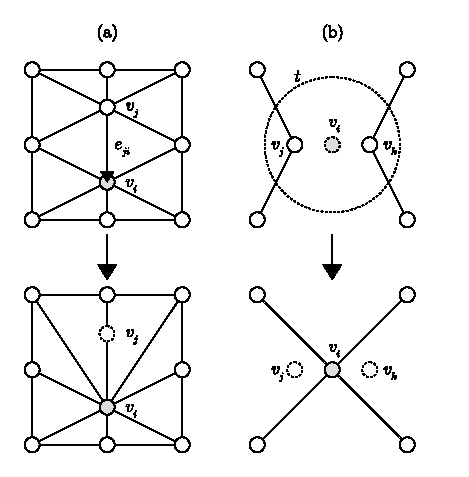
\includegraphics[width=\textwidth]{figures/contraction_types.eps}
        \caption{(a) edge \(e_{ji} = (v_j, v_i)\) contraction towards \(v_i\)
                 and (b) pair \((v_j, v_k)\) contraction in the distance threshold \(t\) toward new vertex \(v_i\).}
        \label{fig:contractions}
    \end{minipage} \hfill
    \begin{minipage}{0.485\textwidth}
        \centering
        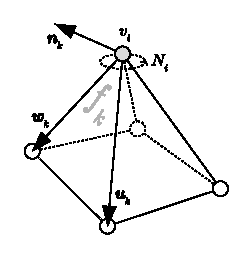
\includegraphics[width=\textwidth]{figures/quadric_planes.eps}
        \caption{depiction of one of the planes \(f_k\) in the neighborhood \(N_i\) of the vertex \(v_i\). It has a normal \(\mathbf{n}_k\); found by the \(\mathbf{w}_k \times \mathbf{u}_k\) of its edges.}
        \label{fig:quadrics}
    \end{minipage}
\end{figure}

\vspace{-0.7em}

Mesh simplification with \emph{Quadric Error Metrics} (QEM), due to \emph{Garland and Heckbert}~\cite{garland1998simplifying}, is based on the vertex merging paradigm. It provides a provably optimal simplification in each iteration, by collapsing the edge \(e_{ji} \rightarrow v_i\) and re-positioning it at \(\mathbf{\bar{v}}\), which gives it the lowest possible geometrical error. By assigning a matrix \(\mathbf{Q}_i\) for each vertex \(v_i\), one can find the error \(\Delta(\mathbf{v})\) introduced by moving \(v_i\) to \(\mathbf{v}\). \(\Delta(\mathbf{v})\) is the sum of distances from \(\mathbf{v}\) to the planes \(\mathbf{f}_k\) in \(v_i\)'s neighborhood \(N_i\) (all polygons around \(v_i\)). Since \(\Delta(\mathbf{v})\) is quadratic, finding a \(\mathbf{v}\) which gives a minimal error is a linear problem. The best position \(\mathbf{\bar{v}}_i\) for \(v_i\) after a collapse \((v_j, v_i) \rightarrow v_i\) is a solution to the eq. \((\mathbf{Q}_j + \mathbf{Q}_i)\mathbf{\bar{v}}_i = \begin{bmatrix} 0 & 0 & 0 & 1 \end{bmatrix}^\intercal\). Thus, according to \emph{Garland and Heckbert}~\cite{garland1998simplifying}:

\[\bar{\mathbf{v}}_i = \begin{bmatrix}
    q_{11} & q_{12} & q_{13} & q_{14}\\
    q_{21} & q_{22} & q_{23} & q_{24}\\
    q_{31} & q_{32} & q_{33} & q_{34}\\
    0 & 0 & 0 & 1\\
\end{bmatrix}^{-1} \begin{bmatrix} 0 \\
                                   0 \\
                                   0 \\
                                   1 \end{bmatrix} \; ,\]

\[\Delta(\mathbf{v}) = \mathbf{v}^\intercal \mathbf{Q}_i  \mathbf{v} \;,\;\; \mathbf{Q}_i = \sum_{f_k \in N_i}  \mathbf{f_k} \mathbf{f_k}^\intercal \; .\]

By storing the \(\Delta(\mathbf{\bar{v}}_i)\) for every valid collapse \(e_{ji} \rightarrow v_i\) in a min-heap, the least cost collapse on the top of the heap can be done in each iteration, removing a vertex in each step. This is repeated until either a user-given vertex count \(|\mathcal{V}|\) is reached or until some error threshold \(\epsilon\).

The results by \emph{Garland and Heckbert}~\cite{garland1998simplifying} show that QEM can reduce the simplification error by up to 50 \% in comparison to a na\"ive scheme where \(\mathbf{\bar{v}}_i = (v_i + v_j) \div 2\) and \(\Delta(\mathbf{v}) = ||\mathbf{v} - v_i||\), as can be seen in Figure~\ref{fig:naive_vs_quadric}. They also argue that QEM gives higher-quality simplifications than \emph{vertex clustering} and that it is faster than \emph{progressive meshing} (which we also present later).

\begin{figure}[h]
    \centering
    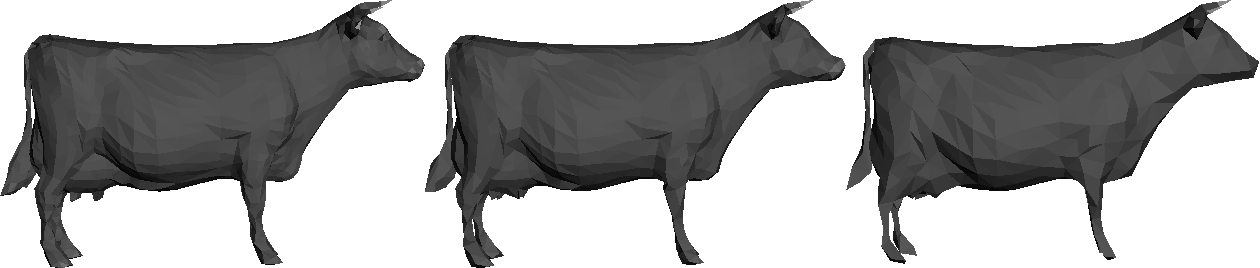
\includegraphics[width=\textwidth]{figures/naive_simplification.png}
    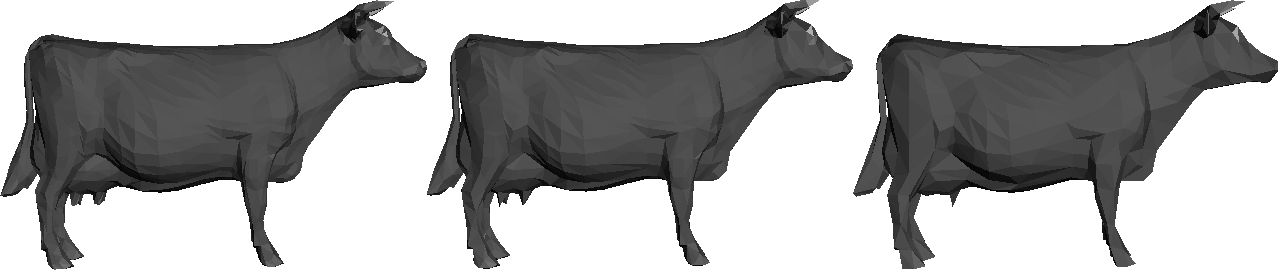
\includegraphics[width=\textwidth]{figures/quadric_simplification.png}
    \caption{simplification using a na\"ive (top image) and a quadric error metric (bottom image) at different levels of detail at some vertex count (left to right: 50 \%, 35 \% and 17 \% of original).}
    \label{fig:naive_vs_quadric}
\end{figure}

\subsection{Appearance-Preserving Simplification} \label{sec:appearance-preserving_simplification}
In order to preserve the appearance of a model when it is simplified, \emph{Cohen et al.} \cite{cohen1998appearance} defines a new \emph{texture deviation metric}. This metric takes three attributes into account: Surface position, surface curvature, and surface color. To properly sample these attributes from the input surface, the surface position is decoupled from the color and normals stored in texture and normal maps, respecticely. The metric guarantees that the maps will not shift more than a user-specified number of pixels on the screen. This user-specified number is defined as $\epsilon$.

Approximation of the surface position is done offline with simplification operations such as edge collapsing and vertex removals. At run-time, the color and normals are sampled in pixel-coordinates with mip-mapping techniques. Mip-maps are a pre-calculated sequence of images with progressively lower resolution. Here the decoupled representation is useful since the texture deviation metric can be used to bound how much the mapped attributes value's positions deviate from the positions of the original mesh. This gurantees that the sampling and mapping to screen-space of the attribues is done in an appropriate way.

Before any simplification can be made, a parametrization of the surface is required in order to store the color and normals in maps. If the input mesh does not have a parametrization, it is created and stored per-vertex in texture and normal maps. Next, the surface and maps are fed into the simplification algorithm which decides which simplification operations to use and in what order. The deviation caused by each operation is measured with the texture deviation metric. A \emph{progressive mesh} (PM) with error bounds for each operation is returned by the algorithm, which can then be used to create a set of LOD with error bounds. Using the error bounds, the tesselation of the model can be adjusted to meet the user-specified error $\epsilon$.

\subsection{Texture Mapped Progressive Meshing} \label{sec:texture_mapped_progressive_meshing}
Given an arbitrary mesh, \emph{Sander et. al} \cite{sander2001texture} presents a method to construct a PM where a texture parametrization is shared between all meshes in a PM sequence. In order to create a texture mapping for a simplified mesh, the original mesh's attributes, e.g normals, is sampled. This method was developed with two goals taken into consideration:
\begin{itemize}
\item{Minimize \emph{texture stretch}:}~~~When a mesh is simplified the texture may be stretched in some areas which decrease the quality of the appearance. Since the texture parametrization determines the sampling density, a balanced parametrization is preferred over one that samples with different density in different areas. The balanced parametrization is obtained by minimizing the largest texture stretch over all points in the domain. No point in the domain will therefore be too stretched and thus making no point undersampled. 
\item{Minimize \emph{texture deviation}:}~~~Conventional methods use geometric error for the mesh simplification. According to the authors this is not appropriate when a mesh is textured. The stricter texture deviation error metric, where the geometric error is measured according to the parametrization, is more appropriate. This is the metric by \emph{Cohen et al.} \cite{cohen1998appearance} explained in Section~\ref{sec:appearance-preserving_simplification}. By plotting a graph of the texture deviation vs the number of faces, the goal is to minimize the height of this graph.
\end{itemize}

\emph{Cohen et al.} \cite{cohen1998appearance} stored an error bound for each vertex in a PM. \emph{Sander et al.} \cite{sander2001texture} instead tries to find an atlas parametrization that minimizes both texture deviation and texture stretch for all meshes in the PM. 

\section{Metrics for Appearance Preservation} \label{sec:metrics_for_appearance_preservation}
Previously in sections \ref{sec:appearance-preserving_simplification} and \ref{sec:texture_mapped_progressive_meshing}, the metrics texture deviation and texture stretch have been defined. But to measure more exactly how much the visual appearance of a simplified mesh deviate from the original mesh another metric would be better. \emph{Lindstrom and Turk} \cite{lindstrom2000image} defines \emph{image-driven simplification} which captures images from different angles of the mesh. The difference between the images of the original and simplified mesh are computed in order to measure how well the appearance is preserved. This metric is more general and can be applied to all simplification algorithms since it only compares the original mesh to the simplified mesh.

The \emph{image metric} is defined as a function taking two images and gives the distance between them. To measure the distance the authors use root mean square of the luminance values of two images $Y^0$ and $Y^1$ with dimensions $m \times n$ pixels. It is defined as:
\begin{equation} \label{eq:rms_images}
  d_{RMS}(Y^0,Y^1) = \sqrt{\tfrac{1}{mn}\sum^m_{i=1}\sum^n_{j=1}(y^0_{ij} - y^1_{ij})^2}
\end{equation}

To evaluate the quality of the simplified mesh the authors capture images from 24 different camera positions. The positions are defined as the vertices of a rhombicuboctahedron which can be seen in figure~\ref{fig:rhombicuboctahedron}. Two sets of $l$ images $Y^0 = {Y^0_h}$ and $Y^1 = {Y^1_h}$ with dimensions $m \times n$ is rendered and the RMS is then computed as:
\begin{equation}  \label{eq:rms_image_sets}
  d_{RMS}(Y^0,Y^1) = \sqrt{\tfrac{1}{lmn}\sum^l_{h=1}\sum^m_{i=1}\sum^n_{j=1}(y^0_{hij} - y^1_{hij})^2}
\end{equation}

\begin{figure}[h]
    \centering
    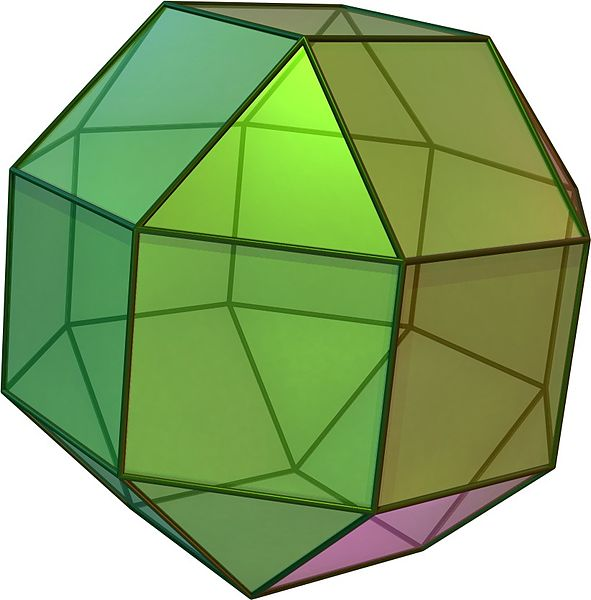
\includegraphics[width=0.25\textwidth]{figures/591px-Rhombicuboctahedron.jpg}
    \caption{Rhombicuboctahedron with 24 vertices which is used as the camera positions. 
      (\href{https://commons.wikimedia.org/wiki/File:Rhombicuboctahedron.jpg}{Rhombicuboctahedron} by Hellisp / \href{https://creativecommons.org/licenses/by/3.0/}{CC BY 3.0})}
    \label{fig:rhombicuboctahedron}
\end{figure}

\section{Measuring Algorithmic Performance} \label{sec:measuring_algorithmic_performance}

According to \emph{David Lilja}~\cite[p.~4]{lilja2005measuring}, there are three fundamental techniques that can be used when confronted with a performance-analysis problem: \emph{measurement}, \emph{simulation} or \emph{modeling}. While the book concentrates on evaluating computer performance, these techniques can also be applied when evaluating different algorithms. Measurement would be to actually execute the implemented algorithm and simultaniously gather interesting statistics (e.g. how long it took to finish and how much memory was needed), and use this to compare the algorithms. While modeling would be to analytically derive an abstract model for the algorithm (e.g. the Big \(\mathcal{O}\) worst-case running time and memory), and see which of them has a lower complexity.

Since not all of the algorithms in Section~\ref{sec:mesh_simplification} have an analytical model derived by the authors, and also because the algorithms are to be evaluated in a real system, only the problems inherent to the measurement approach will be considered. One of the problems with doing measurements of a real system (a program running on a computer in this case), according to \emph{David Lilja}~\cite[p.~43]{lilja2005measuring}, is that they introduce noise. This noise needs to be modeled to be able to reach a correct conclusion, such as determining if algorithm A is faster than algorithm B. One way of doing this, according to \emph{David Lilja}~\cite[p.~48]{lilja2005measuring}, is to find the confidence interval of the measured value, by assuming the source's error is distributed according to some statistical distribution (like the Gaussian or the Student t-distribution). The confidence interval \([a,b]\) when assuming the source's error is t-distributed, can be found as shown below. Where \(n\) tests are taken (giving \(n-1\) degrees of freedom), with a significance level of \(\alpha\) (usually 5 \%).

\[ a = \bar{x} - t_k\frac{s}{\sqrt{n}}, \quad
   b = \bar{x} + t_k\frac{s}{\sqrt{n}}, \quad
   t_k = t_{1-\alpha/2,n-1} \]

One common mistake, according to \emph{Schenker et al.}~\cite{schenker2001judging}, when using confidence intervals to determine if e.g. an implemented algorithm A is faster than B, is the use of the overlapping method to reach conclusions. If two confidence intervals \emph{do not} overlap, then the result is provably significant (that is, algorithm A is either faster or slower than B). However, the converse is not true, if two intervals \emph{do} overlap, then no conclusions can be reached since the result could be either significant or not significant.

%%%%%%%%%%%%%%%%%%%%%%%%%%%%%%%%%%%%%%%%%%%%%%%%%%%%%%%%%%%%%%%%%%%%%%
%%% theory.tex ends here

%%% Local Variables: 
%%% mode: latex
%%% TeX-master: "thesis"
%%% End: 
